\chapter[Synthesis]{Synthesis}
\label{cha:Chapter6}
\newpage

This thesis has contributed towards efforts in large-scale land cover mapping, with an emphasis on the benefits of combining several datasets from different sources and of different types.  It presents different steps of a methodology to extract training data from multiple rich human-annotated datasets and overlay them on Earth observation data from diverse sources, and details the challenges and benefits of doing so while creating land cover maps that navigate the trade-off between spatial, temporal, and thematic resolution, as well as quantity and allocation accuracy.

This thesis, especially in its first two chapters, summarises a relatively 'applied' line of research. Its most important outputs are several datasets that were produced, and have been published as open data (CC-BY):
\begin{enumerate}
    \item 2000-2020 quarterly Landsat composites at 30m resolution and 7 bands;
    \item 2016-2019 quarterly/annual Sentinel-2 composites at 10-30m resolution, depending on the band;
    \item An Ensemble Digital Terrain Model of Europe at 30m resolution;
    \item 2000-2019 annual Land Use / Land Cover maps of Europe at 30m resolution and 43 classes;
    \item Five annual land cover maps of five European countries (Belgium, Czechia, Germany, Luxembourg and The Netherlands) at 30m resolution and 8 classes, whose class proportions match Eurostat area estimates.
\end{enumerate}
The third (and fourth?) chapters describe the later and relatively more innovative attempts to make maps that are faithful to area estimates, and attempts to improve the process of classifying many land cover types with minimal sacrifice of accuracy.

This chapter is divided into two sections: the first summarizes contributions to the research objectives formulated in Section~\ref{sec:research_objectives}; the second reflects on these contributions, offering perspectives on future research opportunities. 

\section{Main Findings}
    The chapters of this thesis each address multiple research questions and have considerable overlap. Their results will be discussed from the perspective of the research questions; each question is discussed below.
    
    \subsection{What are the benefits and challenges of combining multiple large time-series and static EO datasets into Analysis-Ready Data for the purpose of land cover classification?}
    \label{syn:rq1}

        This research question was largely explored in chapters 2 and 3. Chapter 2 details the construction of an Earth observation data cube from several sources (Landsat, Sentinel-2 and several DTMs), and includes experiments that investigate the performance of land cover models using different combinations of these datasets. Chapter 3 uses most of this data cube to train a single LULC classification model, which is subsequently used to create annual maps of Europe between 2000 and 2019. 

        \subsubsection{Benefits}
    
            Our land cover experiments in chapter 2 show that random forest models trained on the largest combination of datasets achieved the highest classification accuracy during cross-validation and that models trained on Landsat and DTM data achieved the highest accuracy on test data.
            This supports the current body of knowledge that using auxiliary information in the feature space can improve performance.
            
            Variable importance of chapter 3 shows that different variables were used by different models
    
            We created an Ensemble DTM which was more accurate than its four source datasets: RMSE 6.544 vs RMSE of 8.451-9.900. This proves that in the case of continuous variables, different versions or representations of that variable can be used as input for a machine learning algorithm, and that the predictions by this algorithm can be more accurate.

        \subsubsection{Challenges}
            
            Experiments in Chapter 2\ref{cha:chapter2} showed that models using the full feature space (Landsat, Sentinel-2 and DTM) achieved the highest classification accuracy, with different datasets improving the results for different land cover classes. This is supported by variable importance in Chapter \ref{cha:chapter3}: Data from four different sources (Landsat, surface water frequency, DTM, and distance to coast) were among the top 15 of 200 variables for LULC modeling.
            
            While it is clear that combining different datasets into one feature space can improve model performance, there are some challenges:
            \begin{itemize}
            \item Differences in spatial resolution
            \item Differences in temporal resolution
            \item Missing data
            \end{itemize}
    
            \textbf{Spatial resolution}
            Overlaying different raster datasets onto training samples may yield high accuracy (like in chapter 2), but can cause artifacts in the shape of low-resolution raster cells creating maps at the highest resolution among the used datasets \citep{moller2019oblique} [SNOWBALL A BIT HERE], or cause low mapping accuracy when mapping at a lower resolution [CITE]. 
            
            \textbf{Temporal resolution}:   
            Which timesteps do you map? Some maps are made by aggregating and averaging observations from several years \citep{pflugmacher2019mapping,esa2023cci}, which may give more robust results than annual maps, but loses detail. In chapters 3 and 4, we chose to make annual maps, and in chapter 3, we made annual maps for each consecutive year. 
        
            We used a space-first predictions strategy throughout this thesis, and not a time-first strategy [CITE GILBERTO?]. This has benefits: [BENEFITS] but also drawbacks. For example, mapping classes that change inside a year, such as crops. There was also considerable confusion between water and wetlands classes in chapter 5
            
            \textbf{Missing Data}:
            This was also seen in chapter 3: While we smoothed out MODIS layers when subsampling to a 30m resolution to avoid artifacts from spatial resolution differences, the land cover maps have gaps near some coastlines due to missing auxiliary layers (see an example \href{https://ecodatacube.eu/?base=OpenStreetMap%20(grayscale)&layer=Land%20Cover%20&zoom=13.2&eye=5000000&center=52.4582,5.3267&opacity=100&time=2019}{here}). We only noticed this much later
    
    
    \subsection{To what extent does training data from multiple times and places improve the accuracy and generalization of land cover classification?}
    \label{syn:rq2}
        Chapters 2 and 3 chapters include experiments that investigate the generalization potential of models trained on data from a single year, and those trained on data from several years. Results from both chapters show that models trained on samples from different years were more accurate; both on years with available training data, and on unseen years.
        
        In the land cover classification experiments of chapter 2, the model that was trained on a small multi-year landsat-only outperformed the model trained on landsat, sentinel, and DTM data on the test set. This suggests there is a unique benefit in training a model on data from a larger time range.
        In chapter 3, 
         In particular, our map of 2017 was validated on the points collected by \citep{jenerowicz2021validation} to validate the S2GLC maps made by \citet{malinowski2020automated}, and achieved a similar accuracy without having training data from 2017 and operating on a lower spatial resolution.
        
        In Chapter \ref{cha:chapter3}, we combined LUCAS points with samples extracted from CORINE polygons to create a training dataset with samples from 8 years (see table \ref{tab:cv_annual}). Cross-validation showed that the weighted F1-score of the model was more consistent through time than through space (with standard deviations of 0.135 per year and 0.150 per 30~km tile, respectively). 

        In Chapter 5, we compare the weighted F1 per NUTS2 area
    
    \subsection{How does the number and type of classes in a legend affect the accuracy of land cover classification?}
    \label{syn:rq3}

        In chapter 3, we found large differences in hard-class accuracy between the three different levels of the CORINE legend: At level 3, only 11 out of 43 classes were mapped with an F1-score above 0.5 (Discontinuous urban fabric, industrial or commercial units, non-irrigated arable land, rice fields, broad-leaved forest, coniferous forest, bare rocks, glaciers and perpetual snow, peat bogs, and water bodies. At level 2, this was 9 out of 14 classes, and at level 1, all 5 classes. At level 3, we can see a positive relationship between the number of samples ('support' in table \ref{tab:cv_accuracy_lvl3}) and the F1-score, although there are classes with many samples that still scored poorly. There is a number of error sources: 

        Firstly, some of these classes are 'mixed types' such as \textit{Complex cultivation patterns}, \textit{Agriculture with significant natural vegetation} and \textit{Mixed forest}. Some other classes occur mostly at a sub-pixel level, in effect being mixed classes with whatever class they border. For instance, \textit{roads and rail networks and associated land} in chapter 3 and the corresponding LUCAS class \textit{Artificial non-built up areas} in chapter 5. Stretches of road or rail infrastructure that are wider than 30~m are relatively rare, and this type of land cover is often very close to other classes such as buildings. If there are classes in the same (level of the) legend, these classes 'compete', even if a prediction for any of them would be true. Second, some LULC classes have the same land cover, but differ in land \textbf{use}, such as \textit{Pasture}, \textit{Natural grasslands}, and \textit{Airports} (which also have significant grasslands, see Figure \ref{fig:airport_grass}). Properly distinguishing those classes may require higher temporal and spectral resolution or feature engineering to detect differences in mowing policy or grass species. 
        
        These mixed class and land use errors largely disappeared when aggregating classes to a level in the hierarchy where mixed nature or land use distinctions ceased to matter, such as \textit{313: Mixed Forests} to \textit{CLC 31: Forests and seminatural areas}. This only works for classes that are placed in a logical order in the legend: For instance, \textit{Pastures} and \textit{Natural grasslands} are considered as completely different LULC types even at the highest level of the legend, where they are aggregated to \textit{Agricultural areas} and \textit{Forest and seminatural areas}, respjectively. In the S2GLC legend, however, we both aggregated these grass classes to \textit{Herbaceous Vegetation}, which was much more effective. This applied to the S2GLC legend in general: When we summed the probabilities of all classes according to the S2GLC scheme, we achieved similar or higher accuracy than the S2GLC land cover maps. This means that training a model on many classes, even more classes than 'needed' for a specific use case, does not need to harm its accuracy in a simpler legend, even when the land cover predictions are inaccurate at the highest thematic level.

        This underlines the necessity of building hierarchical legends that take into account the similarity of classes from a feature space standpoint.
    
        \begin{figure}[H]
        \centering
        \begin{subfigure}[b]{0.6\textwidth}
            \centering
            \caption{Bing imagery}
            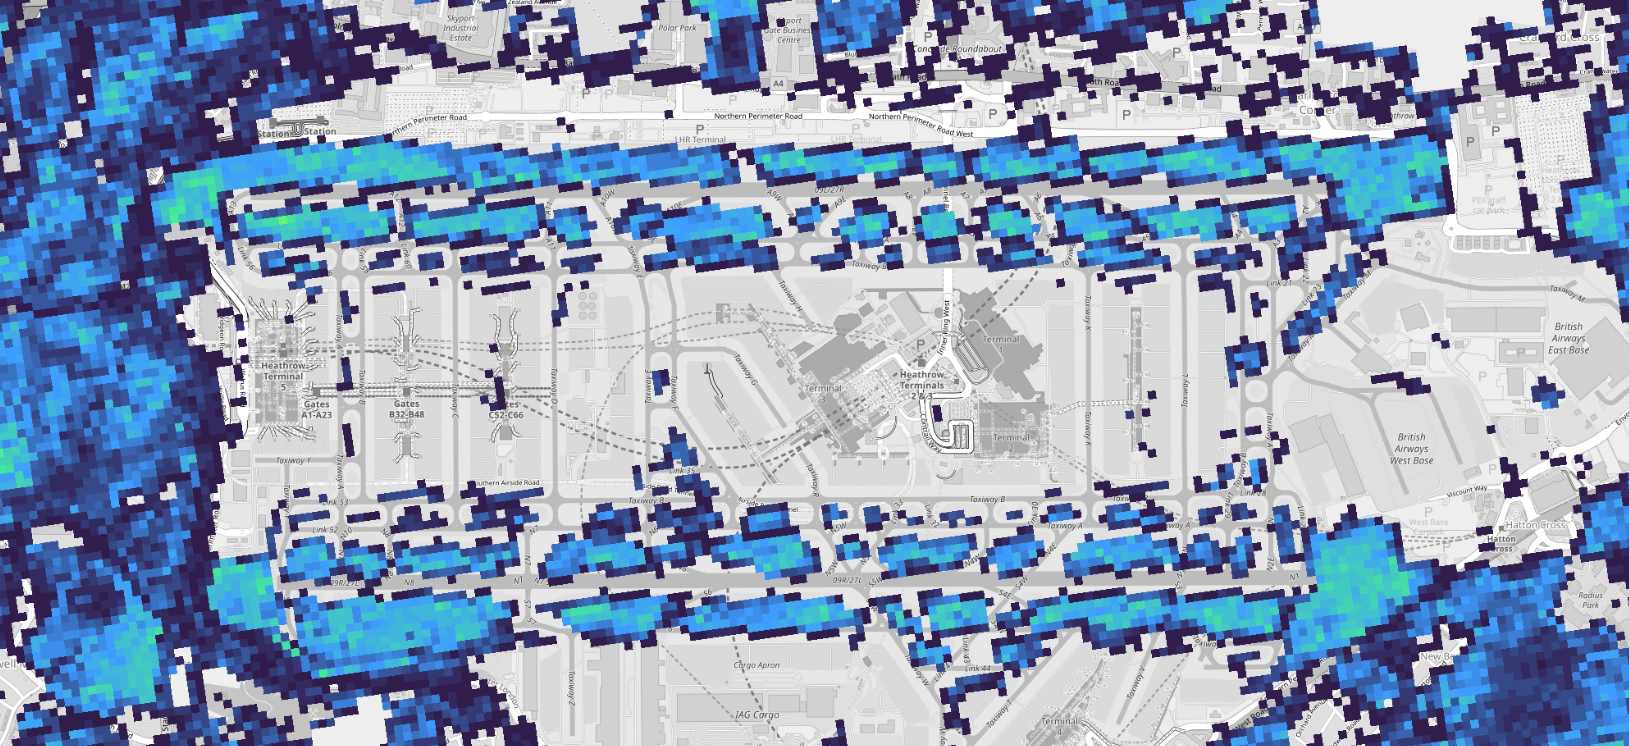
\includegraphics[width=\textwidth]{figs_06/airport_natural_grass.png}
            \label{fig:airport_bing}
        \end{subfigure}
        \begin{subfigure}[b]{0.6\textwidth}
            \centering
            \caption{Probability for \textit{Natural Grass}}
            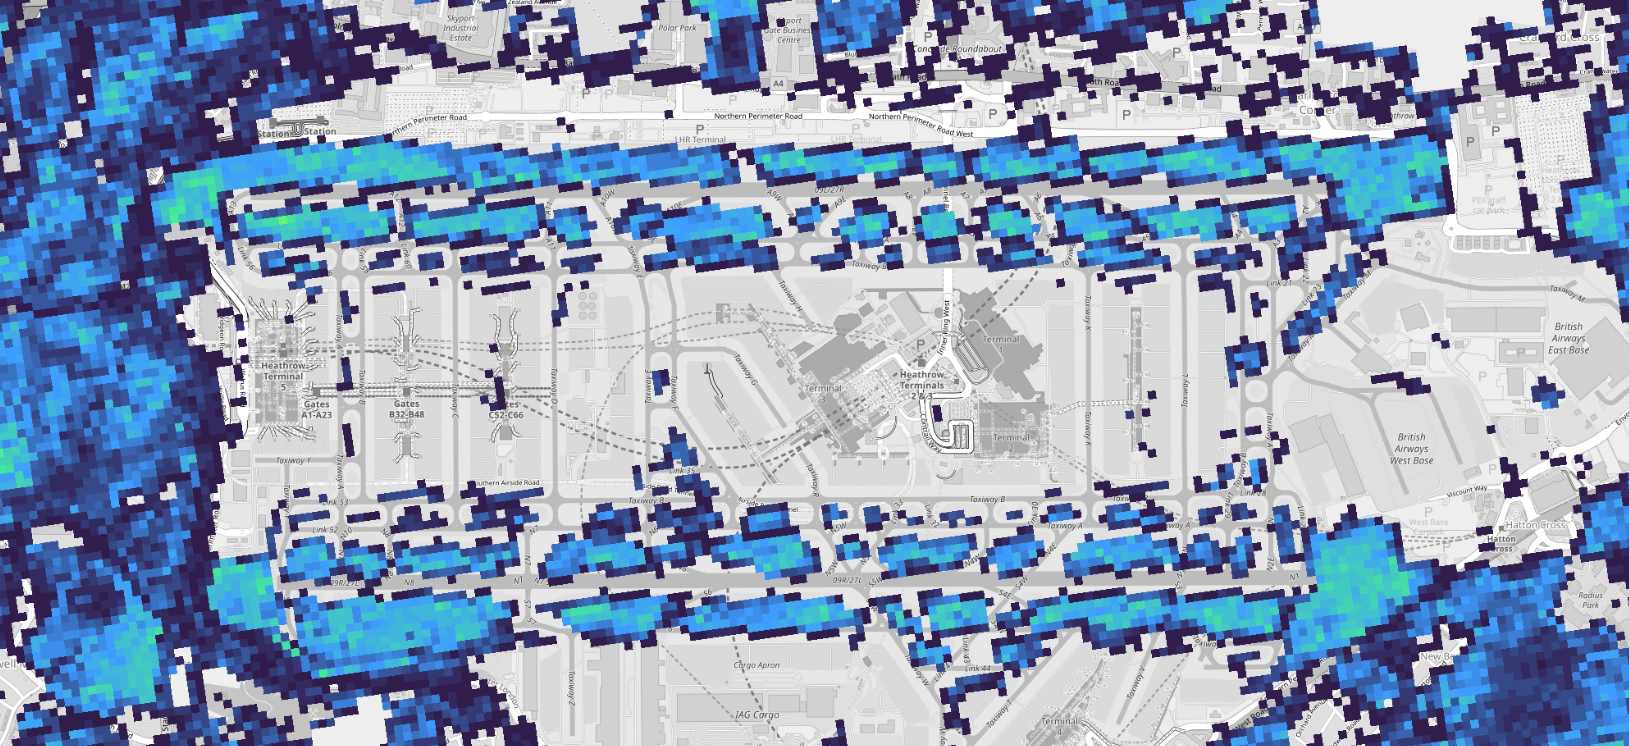
\includegraphics[width=\textwidth]{figs_06/airport_natural_grass.png}
            \label{fig:airport_natural_gras}
        \end{subfigure}
        \begin{subfigure}[b]{0.6\textwidth}
            \centering
            \caption{Probability for \textit{Airport}}
            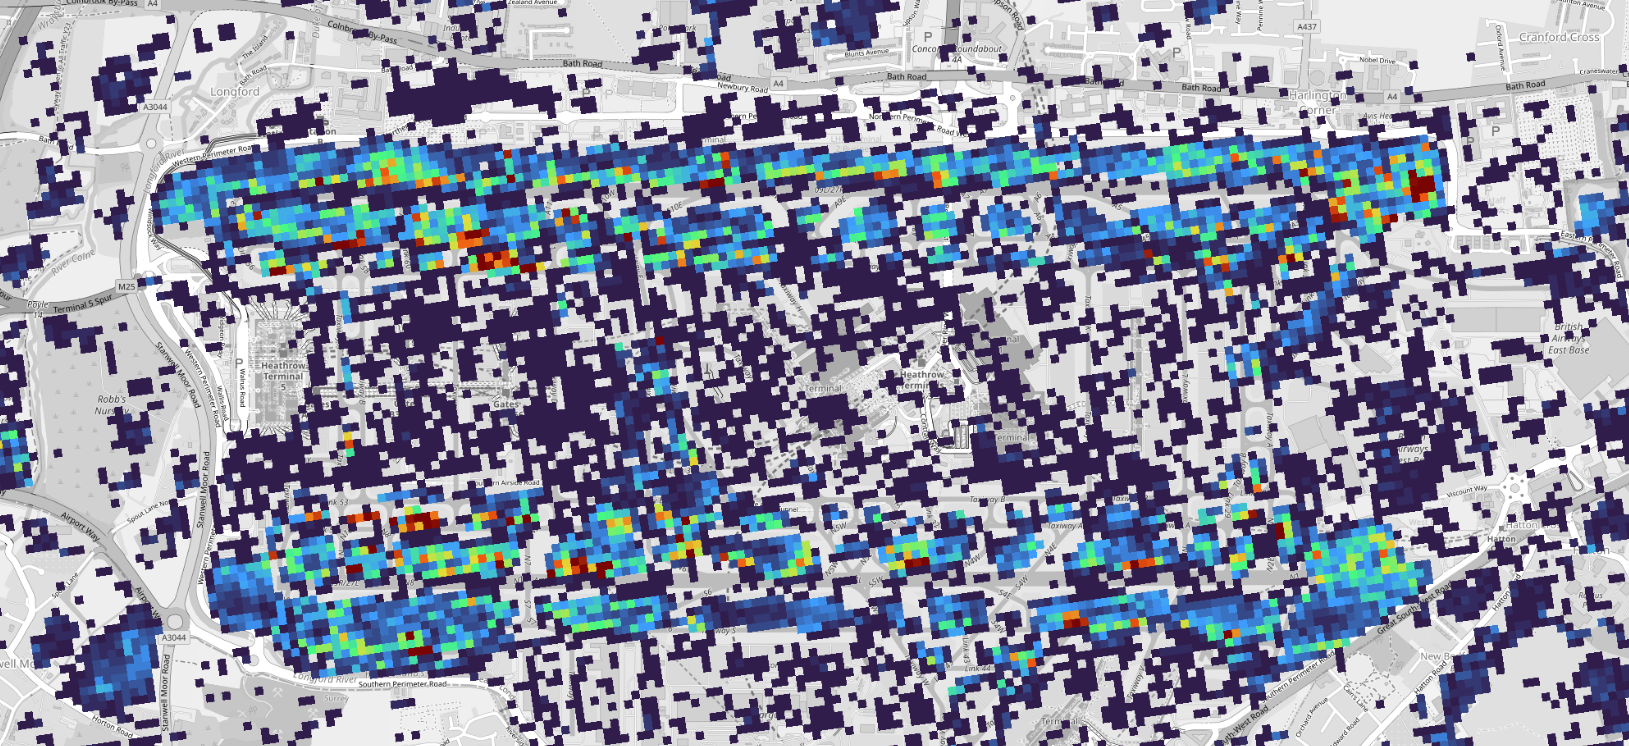
\includegraphics[width=\textwidth]{figs_06/airport_airport.png}
            \label{fig:airport_natural_gras}
        \end{subfigure}
        \begin{subfigure}[b]{0.6\textwidth}
            \centering
            \caption{Probability for \textit{Pastures}}
            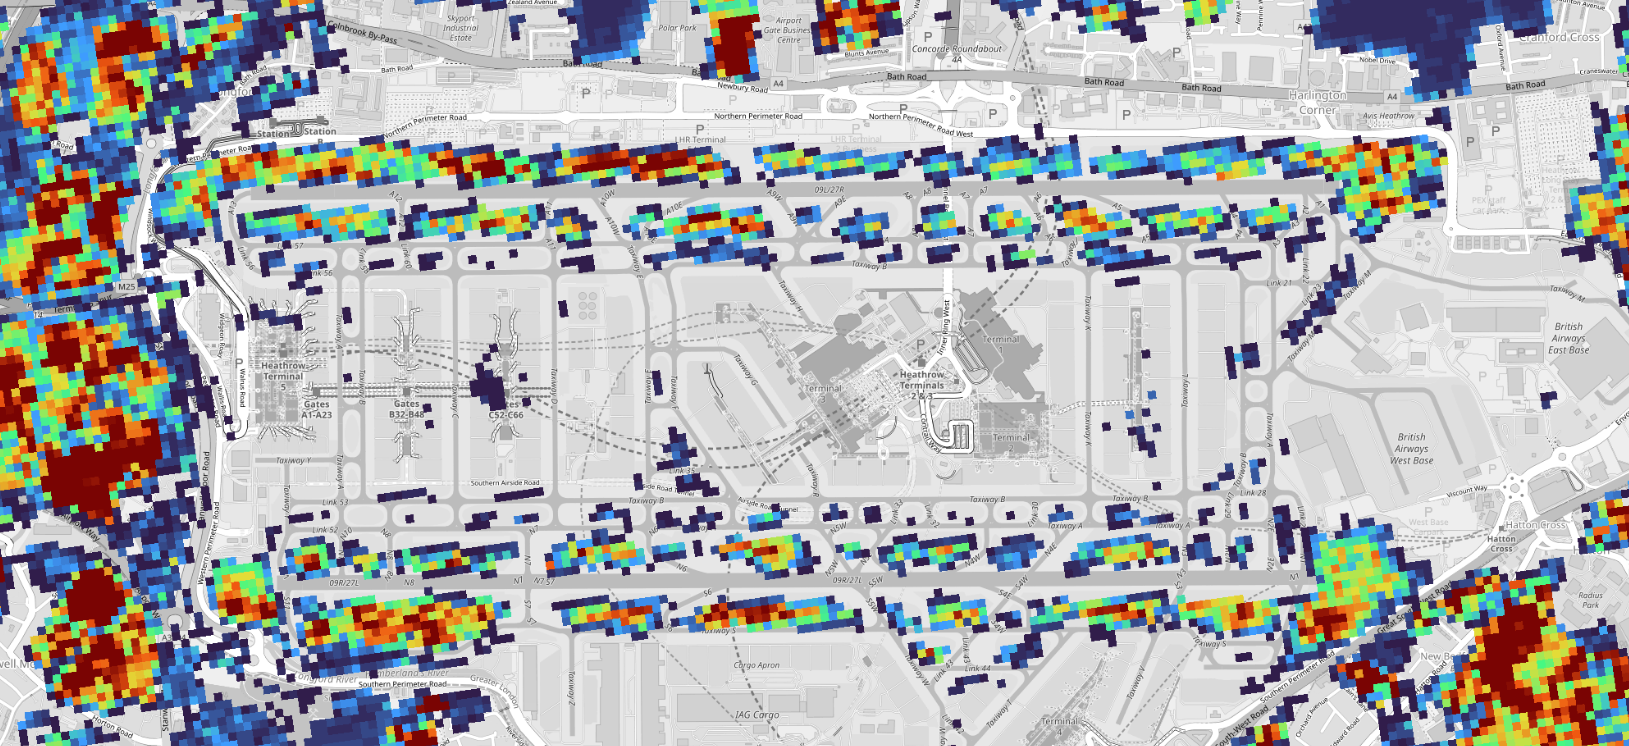
\includegraphics[width=\textwidth]{figs_06/airport_pastures.png}
            \label{fig:airport_natural_gras}
        \end{subfigure}
        \caption{Predicted probabilities for natural grassland, airport, and pastures, for Heathrow Airport, London, in 2019. Note that all three classes closely follow the patterns of the grass fields as seen in the high resolution Bing imagery.}
        \label{fig:airport_grass}
        \end{figure}

        In chapter 5, we used the LUCAS land cover legend instead of the CLC LULC legend. While our main reason was that this allowed us to use area estimates for IMP, it also reduced ambiguity in the legend. While the lack of area estimates for the subclasses of \textit{E: Grassland}, \textit{F: Bare land and lichens/moss}, and \textit{G: Water} limited our legend, the thematic depth of LUCAS and EuroCrops allowed us to closely investigate crop mapping in the same perspective. Here, however, we discovered that when making annual maps with reflectance data, it is very difficult to distinguish crops from grassland. This is likely due to the fact that crops not only have a very different phenology throughout their growing cycle, but also don't cover their 'pixel' the entire year. Instead, many crop fields lie fallow for most of the off-season, and are then covered by herbaceous vegetation. We see this in the consistent confusion of many crop types with the large \textit{Grassland} class.

            %             eml lulc        hsc lc
            %         f1      n       f1  n
            % lvl1    0.83    5       0.74   8
            % lvl2    0.51    14      0.57   19
            % lvl3    0.49    43      0.55   52
            
    \subsection{What is the effect of enforcing correct class proportions on map accuracy?}
    \label{syn:rq4}
    
        Chapters 4 and 5 consistently showed that enforcing correct class proportions with the IMP algorithm can improve map accuracy. In chapter 4, we show that area estimates can be used as input for IMP, which then corrects for bias in the model. This usually comes at the cost of precision (user accuracy) of some classes, while overall gains gains in recall (producer's accuracy) lead to higher weighted F1-scores. This effect is taken to its extreme when validating the land cover model in chapter 5 on calibration points: Instead of area estimates, we used the class counts in the calibration points themselves. Class-wise precision and recall of the IMP classification were identical in each case. 

        Chapter 4 showed that IMP provided a greater accuracy improvement to models that were trained on data with a different class distribution than the area they mapped. This means that IMP can be used to optimize the predictions of large land cover models to a regional context without requiring new training or predictions. It also means that IMP can learn the bias of a model if the model is validated in an area for which class proportions can be estimated; the quantification of this bias can then be stored, and used to make proportional maps of areas for which class proportions are not available. This will require further testing. 
    
    \subsection{Which uncertainty metric is the most useful for optimizing the trade-off between detail and accuracy?}
    \label{syn:rq5}

    [TODO]

    \subsection{Other findings}
    We also have findings that were not part of the research questions:
        
    \subsubsection{Precision, recall, and class proportions}
        
        Section \ref{syn:rq4} briefly mentions that precision and recall were identical for all classes when validating didn't happen with the maps produced and validated for chapter 4: While class-wise precision and recall values of proportional maps were closer to each other than those of maximum probability maps, they were not identical.
    
        While Eurostat area estimates are considered to be quite reliable, a direct class count from a dataset is by definition 100\% accurate. This combination of results suggests that IMP can potentially be used to quantify either how representative a validation dataset is for its study area, or the accuracy of a class proportion (area) estimate. 


\section{Reflection and outlook}

    [MEAT]

    \subsection{Spatiotemporal machine learning}

        Combining several datasets from different times and regions to create large and rich training datasets is a challenging task. It requires knowledge of available data sources, technical skills, and extensive spatial, temporal, and thematic harmonization work. This thesis shows that such a dataset can be used to train a model that classifies many classes. While the accuracy at full thematic depth is lacking compared to those of other recent products, we present proof that the hierarchical nature of complex legends can be leveraged to reach accuracy that is on par with the state of the art. We also show that there are large benefits to training a model on data from different times, even without performing any kind of time-series analysis.

        [Something about the purists and how this is for users with real questions that might not have the means]

        We did not have budget to perform our own validation campaigns.
    
    \subsection{Iterative Mapping of Probabilities}

        The IMP algorithm was developed as an tool to produce maps that match existing area estimates without sacrificing accuracy. We discovered that it can \textit{improve} the accuracy, especially of biased models, because it \textit{learns} the bias in its iterative classwise probability thresholds. The ability of IMP to correct the bias of a model post-hoc also means that models don't need to be trained on datasets that respect class balance. This means it can be combined well with training data generation techniques that don't respect class distributions, such as extracting points from polygons (see chapters 3, 4 and 5). Furthermore, it might improve the usefulness of oversampling techniques such as SMOTE  \citep{chawla2002smote}. While popular for improving minority probability predictions \citep{elor2022smote} and actively researched \citep{douzas2019imbalanced}, SMOTE is critiqued for mostly helping weak classifiers and actively harming the performance of stronger classifiers \citep{elor2022smote}. Oversampling improves the probability predictions of rare classes but worsens majority and overal log loss; this is not an issue when the probabilities are classified with IMP, as it only uses within-class probability distributions.

        \subsubsection{Extrapolating area estimates}
            IMP learns the bias of the model, and quantifies it in the cut-off probability value for each iteration to make sure the bias of the model is countered. This might be generalizable to areas where you don't have area estimates, if the confusion between classes is similar.
            You could store the probability threshold for each class at each iteration, and apply them to probabilities predicted by the same model, for a different area.
            this can be explored by mapping neighboring NUTS2 areas of the ones we have already mapped, using the cutoff values of their originally mapped neighbor. We can then 'pixel count', and compare the counts to the area estimates.

            This could make the method applicable for areas that are less meticulously quantified than Europe.
        
        \subsubsection{Validating area estimates}
            If a reliable, trusted validation data exists for an area, IMP can be used to compare the accuracy of different area estimates by making hard-class maps for each area estimate. The area estimate that matches the reality on the ground most closely should allow IMP to produce the most accurate map.
            In this way, IMP could be used to settle disputes about quantities of land cover and land cover change.

            [example: Forests]

        \subsubsection{Wider applicability}
        
            Land cover and other remote sensing fields are not the only potential application for IMP. It can be used for any type of machine learning task where class proportions can be either estimated or targeted, and where bias must be quantified. Any field that utilizes machine learning models and faces challenges with class imbalance, representation bias, or requires models to perform accurately across diverse and potentially underrepresented group, could use the algorithm to enhance model fairness, accuracy, and generalization.

            In medical diagnosis and disease prediction models, data can be inherently biased due to uneven representation of disease cases across populations. An algorithm that corrects for such biases could improve the accuracy of diagnostic tools and predictive models, making them more reliable for clinical decision-making and research studies. For instance, it could help in developing more accurate models for rare disease diagnosis where the class imbalance is a significant issue \citep{weiss2004mining,krawczyk2016learning}.

            Financial institutions often use machine learning models for credit scoring and risk assessment. The training data can be biased due to historical decisions and social demographics, potentially leading to unfair assessments. A post-hoc correction algorithm could mitigate these biases, leading to fairer credit scoring and risk assessment models \citep{chen2018why, kamiran2012data}.

            In predictive policing and recidivism prediction, biases in the training data can perpetuate and amplify societal biases. An algorithm that adjusts predictions post-hoc could help in reducing the bias in such models, contributing to fairer decision-making in the criminal justice system \citep{berk2021fairness, dressel2018accuracy}.

            Recommendation systems in retail often suffer from popularity bias, where popular items are more likely to be recommended, potentially ignoring the long tail of less popular items. An algorithm that can correct for such biases post-hoc would improve the diversity and fairness of recommendations \citep{abdollahpouri2019managing}.
    
    
    \subsection{Hierarchical Selective Classification}
    
        Selective hierarchical classification will be more fine-grained if you have more levels in your hierarchy.
        Eurostat should publish more detailed area estimates and include LULC combinations. There is plenty of training data available for e.g. pastures, natural grasslands, and other grass areas such as those near airports.

        \subsubsection{Prediction uncertainty}
        
            Finding the best uncertainty metric will be helpful. Well-calibrated probabilities and the margin of victory \citep{calderon-loor2021high} can be used as a heuristic proxy but offer no statistical guarantee. The land cover community is exploring techniques that promise such statistical guarantees on uncertainty quantification, such as conformal prediction \citep{angelopoulos2023predictionpowered,valle2023quantifying,singh2024uncertainty}. So far, however, they remain unused by the large-scale mapping initiatives, although those that publish all probabilities (like DynamicWorld) allow users to calculate some metrics themselves [CITE who did that]
        
            IMP: Classifications in earlier iterations are much more accurate than later classifications. The user accuracy on calibration data (from the same source as the training data) is a robust indicator of relative accuracy, which then can be regularized using the final validation of the map with an independent test dataset (e.g. LUCAS).
    
        \subsubsection{Best models for the job}
                Can you train models in such a way that they are relatively more likely to make mistakes within the same category? Iterative learning models, such as gradient boosting and neural networks, might be trained with custom loss functions.

    % \subsection{Transfer learning and Foundational Models}
    
    
    \subsection{Reflection: do we really need these maps? What kind of maps do we really need?}

    maps without users are meaningless
    wrong maps with users are dangerous \citep{bastin2019global}
    good maps with the wrong users are even more dangerous: 
    Poachers \citep{beery2021can}- 
    soil carbon, food and beverage companies are looking to reduce their carbon footprint  want to keep polluting. Disaster analysis maps are used by investors and insurance companies, buying land. Poachers etc. Do farmers benefit from cropland maps? No.
    Exponential benefit to those who are already rich and powerful.
    
    Spatial resolution:
        
    temporal resolution:
    crop mapping annually is difficult: you need sub-annual maps to do it properly. But where does this end? Daily maps? Multiple satellites flying in 
    
    \subsection{Reflection: Open Data}
    mention cool suppliers of open data:
Major TOM \citep{francis2024major}
    https://radiant.earth/blog/2023/05/we-dont-talk-about-open-data/ (the case against open data: helping poachers etc.)
    \subsection{Future maps}
    
        People are working on reproducing CORINE with ML, allbeit at 14 classes \citep{bhugra2022rapidai4eo}

        It would be great if area estimates were available for all LUCAS land cover and land use combinations. IMP can help validate them!

        Mention EAGLE legend

        
        It is important to validate annual large-scale maps with up-to date validation data to ensure there is no dataset drift and to properly quantify accuracy and uncertainty \citep{tsendbazar2021towards}
    
    
            
                
            



        

